\section{From Resources to Systems: What Each Graph Enables}
\label{sec:enables}

Section~\ref{sec:resources} described the graphs as data. This section asks the question an engineer actually starts with: given a particular graph and a particular clinical or scientific task, what can be built on it, what has already been built, and what does its structure make possible that a flat text index does not? The framing matters because graph choice is not a neutral preliminary. It fixes which retrieval mechanisms are expressible, which agent actions are meaningful, and which failure modes the system inherits.

\subsection{Structure determines the retrieval mechanism}

Modern retrieval-augmented generation offers a standard toolkit: dense passage retrieval, sparse lexical matching, hybrid fusion, cross-encoder reranking, query decomposition, hypothetical document expansion, and iterative or corrective loops that re-retrieve when the first attempt looks insufficient. Applied to a graph, each of these behaves differently depending on what the graph actually encodes, and the difference is not cosmetic.

\emph{Typed edges make relation-constrained retrieval expressible.} SPOKE distinguishes 21 node and 55 edge types~\cite{morris2023spoke}. A query that needs ``drugs that target a protein in this pathway but are not contraindicated in renal impairment'' is a typed traversal with a negative constraint. A dense index over verbalized triples cannot express the constraint; it can only hope that semantic similarity approximates it. The engineering consequence is that graphs with rich edge typing reward symbolic or hybrid retrieval, while schema-light graphs push you toward embedding similarity and therefore toward all of its failure modes.

\emph{Evidence-bearing edges make provenance-first ranking possible.} iKraph carries relations from all PubMed abstracts alongside database-derived assertions and probabilistic inference~\cite{zhang2025ikraph}, and MDKG attaches conditional statements, cohort characteristics, source, and confidence to each relation~\cite{gao2025mdkg}. On such a graph, retrieval can rank by evidence strength rather than by embedding proximity, and it can return supporting and contradicting evidence as separate result sets. On a graph without assertion-level provenance, neither is available, and a system built there cannot honestly implement claim-level attribution no matter how good its generator is.

\emph{Semantic distinctions in the schema make safety-relevant retrieval possible.} PrimeKG separates indications, contraindications, and off-label uses~\cite{chandak2023primekg}. That single design choice is what allows a retriever to be evaluated on contraindication recall, which for a prescribing-support task matters more than aggregate accuracy. A graph that collapses these into a generic \emph{drug--disease} relation cannot support the evaluation, so the safety property becomes unmeasurable rather than merely unmet. Frequency-based traversal over such typed relations can classify a drug's effect on a disease without any learned model at all~\cite{chanda2026drugeffect}.

\emph{Hierarchy and community structure make global questions tractable.} Path retrieval answers local, relation-specific questions well and broad synthesis questions poorly. Community detection over a large graph, following the pattern established for query-focused summarization~\cite{edge2024graphrag}, gives a retriever something to return when the question has no single decisive path. KARE exploits exactly this on a multi-source concept graph~\cite{jiang2025kare}, and MedRAG builds a purpose-shaped four-tier hierarchy so that retrieval discriminates among diseases with overlapping presentations rather than merely finding similar text~\cite{zhao2025medrag}.

\emph{Attribute-rich nodes make cross-modal retrieval possible.} PrimeKG++ and BioMedKG add textual descriptions, SMILES strings, and amino-acid and nucleotide sequences to graph nodes~\cite{dang2025biomedkg}. This turns the graph into an alignment substrate: retrieval can cross from a molecule to a protein to a disease phenotype through learned transformations rather than through text alone, which is the mechanism BioBridge formalizes~\cite{wang2024biobridge}. Multimodal transformers can then predict a drug's mechanism of action directly from these aligned representations~\cite{das2025drugmap}.

\subsection{What has been built, and on what}

Table~\ref{tab:enables} joins graphs to the systems built on them, the retrieval mechanism each uses, and the agentic capability each demonstrates. Two features of the table are worth reading deliberately. First, several widely cited graphs have no agentic system built on them at all, which marks the clearest near-term opportunity in the field. Second, a number of systems do not state which graph snapshot they used, and the table records that rather than inferring it; unreported provenance is a finding about the literature, not a gap in the table.

\begin{table*}[!t]
\centering
\caption{\textbf{Which systems have been built on which graph, and what each graph would additionally support.} This table joins the resources of Section~\ref{sec:resources} to the methods of Sections~\ref{sec:kgtollm} onward, so that a reader starting from a chosen graph can find the closest prior work. ``Agentic capability'' means the system chooses among actions based on intermediate results rather than following a fixed sequence; a pipeline that always links, retrieves, then generates is not agentic even when every stage calls a model. ``Not reported'' records that the source paper does not state its graph snapshot, which is itself a finding about the literature. The empty and orange cells are the most informative part: the final row lists three widely used graphs that carry the provenance and temporal metadata an agent needs and on which no agentic system has been built.}
\label{tab:enables}
\footnotesize
\begin{tabularx}{\textwidth}{@{}L{2.1cm} L{2.7cm} L{3.2cm} L{2.6cm} Y@{}}
\toprule
\textbf{Graph} & \textbf{Systems built on it} & \textbf{Retrieval mechanism} & \textbf{Agentic capability} & \textbf{What the structure additionally unlocks} \\
\midrule
SPOKE~\cite{morris2023spoke} & KG-RAG~\cite{soman2024kgrag} & Prompt-aware context extraction with embedding-based pruning & None; single-pass retrieval & Typed multi-hop traversal with negative constraints; cross-scale queries from variant to phenotype to drug \\
UMLS~\cite{umls} & DR.KNOWS~\cite{zuo2025drknows}, medIKAL~\cite{jia2025medikal}, ILlama~\cite{park2025illama} & Path ranking via GNN and path encoder; typed entity weighting; precomputed triple documents & Iterative path expansion toward diagnosis concepts & Concept normalization as a shared interface across sites; assertion-status-aware patient graphs \\
PrimeKG~\cite{chandak2023primekg} & MHGraphBench tasks~\cite{liu2026mhgraphbench}; controlled retrieval study~\cite{mandarapu2026controlled} & Snippet injection; counterfactual-controlled retrieval & None reported & Contraindication-aware retrieval and evaluation; ten-scale reasoning; drug repurposing with explicit indication semantics \\
Hetionet / DRKG~\cite{himmelstein2017hetionet,ioannidis2020drkg} & Metapath filtering~\cite{ratajczak2022metapath} & Task-driven metapath selection & None; graph-native prediction & Learned metapath priors as an agent tool; hypothesis ranking with leakage-controlled splits \\
Multi-source concept graph & KARE~\cite{jiang2025kare} & Hierarchical community retrieval plus patient-context augmentation & Reasoning-trace distillation, not run-time agency & Community summaries as an agent's coarse index before path-level drill-down \\
Four-tier diagnostic hierarchy & MedRAG~\cite{zhao2025medrag} & Hierarchical discrimination plus similar-EHR retrieval & Follow-up question generation & Differential-diagnosis narrowing as an explicit agent objective \\
User docs plus authoritative sources & MedGraphRAG~\cite{wu2025medgraphrag} & Top-down precise retrieval with bottom-up refinement & Two-stage refinement loop & Claim-level entailment checking against the linked source layer \\
AlzKB & ESCARGOT~\cite{matsumoto2025escargot} & Executable graph-of-thought with graph queries & Plan, execute, inspect over a disease graph & Template for disease-specific agentic discovery on other curated graphs \\
Chemical reaction KG & KGRxn-LLM~\cite{liu2026kgrxn} & Agentic retrieval over a four-level hierarchy & Full agent loop with covered/holdout evaluation & The clearest existing model for separating graph-covered from generalization performance \\
Oncology KG (proprietary) & Trial matching~\cite{loaizabonilla2026trialmatch} & Ontology normalization plus deterministic eligibility rules & Multi-agent extraction then reasoning, with clinician review & Deterministic arbitration over agent output; the strongest clinical-stage precedent \\
Self-built medical KG & AMG-RAG~\cite{rezaei2025amgrag} & Continuous construction with current-evidence retrieval & Construction, update, and retrieval agents & Automated maintenance; also the largest untested risk surface \\
iKraph~\cite{zhang2025ikraph}, PubMedKG 2.0~\cite{xu2025pubmedkg}, CKG~\cite{santos2022ckg} & None identified & --- & None & Provenance-ranked retrieval; trial-aware and patent-aware evidence tracing; multi-omics agent tools \\
\bottomrule
\end{tabularx}
\end{table*}

\subsection{Where the opportunities sit}

Reading the table by its empty cells is more informative than reading it by its entries. Three gaps stand out, and one caution applies to all of them: several of these graphs share upstream sources, as Fig.~\ref{fig:provenance} shows, so results replicated across them are less independent than a count of graphs implies.

% How the representative graphs relate through shared upstream sources.
\begin{figure}[!t]
\centering
\resizebox{\columnwidth}{!}{%
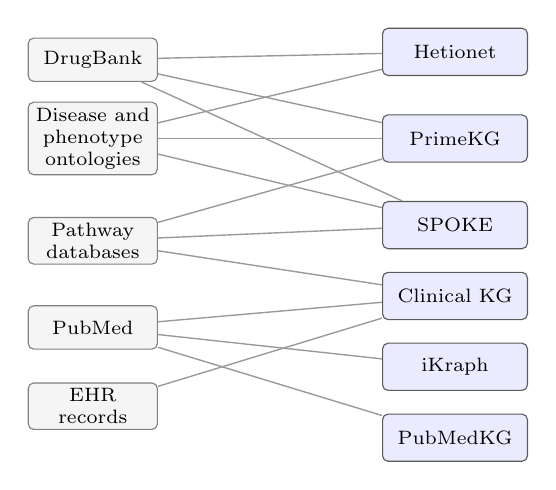
\begin{tikzpicture}[
  font=\scriptsize,
  src/.style={draw=black!50, rounded corners=2pt, fill=black!4,
              align=center, inner sep=2pt, text width=15mm, minimum height=5.5mm},
  kg/.style={draw=black!65, rounded corners=2pt, fill=blue!8,
             align=center, inner sep=2pt, text width=17mm, minimum height=6mm},
  e/.style={draw=black!40, line width=0.5pt}
]

% upstream sources
\node[src] (drugbank) at (0,0)      {DrugBank};
\node[src] (diseaseont) at (0,-1.0) {Disease and phenotype ontologies};
\node[src] (pathway) at (0,-2.3)    {Pathway databases};
\node[src] (pubmed) at (0,-3.4)     {PubMed};
\node[src] (ehr) at (0,-4.4)        {EHR records};

% derived graphs
\node[kg] (hetio) at (4.6,0.1)   {Hetionet};
\node[kg] (primekg) at (4.6,-1.0) {PrimeKG};
\node[kg] (spoke) at (4.6,-2.1)  {SPOKE};
\node[kg] (ckg) at (4.6,-3.0)    {Clinical KG};
\node[kg] (ikraph) at (4.6,-3.9) {iKraph};
\node[kg] (pkg) at (4.6,-4.8)    {PubMedKG};

% edges: shared provenance
\draw[e] (drugbank) -- (hetio);
\draw[e] (drugbank) -- (primekg);
\draw[e] (drugbank) -- (spoke);
\draw[e] (diseaseont) -- (hetio);
\draw[e] (diseaseont) -- (primekg);
\draw[e] (diseaseont) -- (spoke);
\draw[e] (pathway) -- (spoke);
\draw[e] (pathway) -- (ckg);
\draw[e] (pathway) -- (primekg);
\draw[e] (pubmed) -- (ikraph);
\draw[e] (pubmed) -- (pkg);
\draw[e] (pubmed) -- (ckg);
\draw[e] (ehr) -- (ckg);

\end{tikzpicture}%
}
\caption{Shared provenance among the representative graphs. Because several draw on the same upstream databases, two evaluations that use different graphs are not necessarily independent: an error or bias in DrugBank or in a disease ontology propagates into Hetionet, PrimeKG, and SPOKE alike. A result replicated across graphs that share sources is weaker evidence than the count of graphs suggests.}
\label{fig:provenance}
\end{figure}


The large literature-scale and multi-omics graphs, iKraph, PubMedKG 2.0, and the Clinical Knowledge Graph, carry exactly the properties an agent needs, namely resolvable provenance, temporal metadata, and links between assertions and the documents or experiments that support them, and yet no agentic system in the reviewed literature is built on them. An agent over PubMedKG 2.0 could trace a claim from a guideline to the trials that support it to the patents that surround it, which is a translational-evidence workflow no current system performs. The obstacle is engineering effort rather than any missing capability.

Contraindication-aware retrieval is expressible on PrimeKG and is not being evaluated. The graph makes the distinction available, the safety case for using it is obvious, and the reviewed systems still report aggregate accuracy. This is a case where a measurable safety property is going unmeasured because the evaluation convention has not caught up with the data.

Deterministic arbitration over agent output has one strong precedent~\cite{loaizabonilla2026trialmatch} and one clear architectural argument in its favor~\cite{wang2026crossddi}, and it remains rare. A deterministic Graph-RAG approach to drug--disease association discovery applies the same principle, replacing the generative arbiter with an auditable graph procedure~\cite{pramanik2026mechanistic}. For any task where eligibility, dosing, or interaction can be expressed as a rule, letting agents gather evidence and letting a deterministic component decide is both more auditable and more stable across model versions than asking a generator to arbitrate.

\subsection{Choosing a configuration for a task}

The preceding analysis supports a short design path. Start from the question type. Relation-specific and mechanistic questions want typed path retrieval on a schema-rich graph. Broad synthesis and patient-context enrichment want community or hierarchical retrieval. Questions turning on qualifiers, dose, population, or study design want hybrid graph-and-text retrieval, because a triple will not carry those and a passage will. Questions answerable by an exact constraint want symbolic query execution with the model confined to translating the question, and an eligibility or interaction decision wants a deterministic arbiter rather than a generator.

Then check three properties of the candidate graph before committing: whether it contains the decisive entities and relations for the target cohort, whether it carries assertion-level provenance if the output must be attributable, and whether its update cadence matches how fast the underlying knowledge moves. A graph that fails the first is the wrong graph. A graph that fails the second forecloses claim-level attribution regardless of what the generator does. A graph that fails the third will be confidently wrong about anything recent, and no retrieval mechanism repairs that.
